% =====================================================================
%  CSC_43M04_EP — Computer Vision with Deep Learning (École Polytechnique)
%  Team 8 — Florian Guillaumey & Andrea Signoretti
%  Report (merged): unified two-track report (Closed World + Open World),
%  Track~A section refreshed with the ResNet50 backbone and ablation results.
%
%  CVPR double-column template. Requires cvpr.sty + ieeenat_fullname.bst
%  (already in docs/). silence.sty and cleveref.sty stubs are provided for
%  TeX installs that lack them.
%
%  Build (from docs/report_merged/):
%    export TEXINPUTS="$PWD:" BSTINPUTS="$PWD:" BIBINPUTS="$PWD:"
%    pdflatex report && bibtex report && pdflatex report && pdflatex report
%
%  Figures live in figures/ and are gathered at the END after \clearpage.
% =====================================================================
\documentclass[10pt,twocolumn,letterpaper]{article}

\usepackage{cvpr}              % final (camera-ready) mode
\usepackage{graphicx}
\usepackage{amsmath,amssymb}
\usepackage{booktabs}
\usepackage{xcolor}
\usepackage[pagebackref,breaklinks,colorlinks,allcolors=blue]{hyperref}

\graphicspath{{figures/}}

\def\cvprPaperID{8}
\def\confName{CSC\_43M04\_EP — Modal d'informatique}
\def\confYear{2026}

\title{What Happens Next? Closed- and Open-World Video Action Recognition\\
on a 33-Class Something-Something\,V2 Subset}

\author{%
Florian Guillaumey\\
École Polytechnique --- Team 8\\
{\tt\small florian.guillaumey@polytechnique.edu}
\and
Andrea Signoretti\\
École Polytechnique --- Team 8\\
{\tt\small andrea.signoretti@polytechnique.edu}
}

\begin{document}
\maketitle
\thispagestyle{plain}
\pagestyle{plain}
\vspace{-1.2em}
\begin{center}\small June 8, 2026\end{center}

% =====================================================================
\begin{abstract}
We present a two-track study of temporal action prediction on a 33-class subset
of Something-Something\,V2 (SSv2)~\cite{goyal2017ssv2}, ``What Happens Next?'':
only the first ${\approx}40\%$ of each clip (four JPEG frames) is given, so the
outcome is withheld and classification must reason about motion. In
\textbf{Track~A (Closed World)}, where pretraining is forbidden, our study shows that
\emph{where} a model mixes time matters more than \emph{how much} capacity it
has: Temporal-Shift-Module~\cite{lin2019tsm} (TSM), which mixes frames
\emph{before} spatial pooling, beats VideoFormer-Lite (VFL, global
post-pooling attention) by $+3.0$\,pp at matched backbone size, and scaling
its backbone from ResNet18 to ResNet50 then adds a further $+3.4$\,pp to reach
\textbf{42.85\%} \texttt{val\_dir} (our best single model). A five-model
log-softmax ensemble of TSM and VFL variants with test-time augmentation
reaches \textbf{46.75\%} \texttt{val\_dir} and \textbf{0.4785} public /
\textbf{0.4547} private on Kaggle --- our best closed-track submission. In
\textbf{Track~B (Open World)}, we fine-tune V-JEPA\,2~\cite{bardes2025vjepa2}
and VideoMAE~\cite{tong2022videomae} backbones with progressive unfreezing,
layer-wise learning-rate decay, window-capped source-frame re-extraction and
pseudo-labelling, then build a 14-model uniform ensemble reaching
\textbf{0.6586} Kaggle top-1 (16th in both tracks). We document a
self-discovered data-leakage event (a discarded 0.81 submission) and show that
ensemble diversity across architecture families beats single-family or
learned-weight ensembling. Failure analysis attributes the residual errors to
real-vs-pretended and direction-ambiguous classes that four frames
under-determine.
\end{abstract}

% =====================================================================
\section{Problem Description}
\label{sec:problem}

\paragraph{Task.}
The challenge classifies four-frame JPEG clips into one of 33 motion-defined
action classes (e.g.\ \emph{Pouring something into something}, \emph{Pulling
something from left to right}). Crucially, each clip contains only the
\emph{anticipatory} portion of the source SSv2 video---the shipped
\texttt{frame\_003} sits at a median fraction of $0.40$ of the source clip---so
the action's outcome is deliberately withheld and the task probes motion
prediction, not final-state recognition~\cite{goyal2017ssv2}.

\paragraph{Dataset.}
The split provides $44{,}993$ training clips, $6{,}745$ validation clips and
$6{,}913$ test clips over 33 classes (numeric prefixes 000--032; class~027 is
absent from training). Classes are heavily imbalanced: the largest (009,
\emph{Moving something up}) has $3{,}170$ examples while the smallest (026,
\emph{Spilling something next to something}) has only 162, a ratio of
$19.6\times$. The KL divergence between training and validation class
distributions is $0.088$, confirming the splits are representative.

\paragraph{Evaluation and tracks.}
Submissions are scored by top-1 accuracy on a public+private Kaggle leaderboard
over two stages (Stage~1, intermediate; Stage~2, final); top-5 is tracked
internally. The provided baseline reaches ${\approx}0.55$ private and the
second-place public reference is $0.74$; our final submissions placed
\textbf{16th in both tracks} (counting the multiple accounts fielded by some
teams). Following the challenge, we report two regimes. \textbf{Track~A (Closed
World)} prohibits pretrained models and external data---all spatial features,
temporal dynamics and class boundaries are learned from scratch on the four
provided frames. \textbf{Track~B (Open World)} permits pretrained backbones and
external corpora but not future frames or test labels. The task is hard for
three reasons: (i)~labels are motion-defined, defeating appearance-only
models~\cite{goyal2017ssv2}; (ii)~four frames is an order of magnitude below the
8--32 standard in video recognition~\cite{lin2019tsm,bertasius2021timesformer};
(iii)~the discriminative cue---the action's outcome---is withheld by
construction.

% =====================================================================
\section{Methods}
\label{sec:method}

\subsection{Track A --- Closed World}
\label{sec:trackA}
The pipeline evolved through several iterations on an internal training-split,
all trained from scratch (the closed track forbids pretraining and external
data). Our guiding hypothesis is that, without pretraining, \emph{every
parameter spent on temporal modelling is one not spent learning spatial
features}, favouring parameter-free temporal mechanisms over heavy temporal
heads --- and that \emph{where} in the network temporal information is mixed
matters as much as how it is mixed.

\subsubsection{Architecture family and complexity}
\label{sec:arch}
All three Track~A architectures share the contract $(B, T, C, H, W) \to
(B, 33)$ with $T{=}4$, $H{=}W{=}224$, and a ResNet
backbone~\cite{he2016resnet} mapping each frame to a $512$-d (R18) or
$2048$-d (R50) vector after global average pooling. \textbf{CNNBaseline} and
\textbf{CNN-LSTM} simply average (resp.\ recurrently combine) the $T$ pooled
features --- weak baselines ($\approx\!11.2$\,M params) since BPTT on
four-step sequences barely helps. The two strong families differ in
\emph{where} they mix time relative to spatial pooling.

\noindent\textbf{TSM-ResNet}~\cite{lin2019tsm} re-indexes, \emph{inside every
residual block and before every convolution}, a fraction
$1/\text{fold\_div}$ of channels one step backward and another
$1/\text{fold\_div}$ one step forward in time:
\begin{equation}
  \text{TSM}(\mathbf{x})_{t,c} = \begin{cases}
  \mathbf{x}_{t-1,c} & c < C/4 \\
  \mathbf{x}_{t+1,c} & C/4 \leq c < C/2 \\
  \mathbf{x}_{t,c}   & \text{otherwise,}
  \end{cases}
  \label{eq:tsm}
\end{equation}
at \emph{zero} parameter cost, while spatial resolution is still full. The $T$
final per-frame vectors are averaged and a linear head $d\!\times\!33$ yields
the logits, so the total cost is exactly backbone $+$ head:
$\approx\!11.2$\,M (R18) and $\approx\!23.6$\,M (R50, $23.5$\,M of which is the
backbone). TSM was designed for SSv2-style motion labels and is a strong prior
here (Fig.~\ref{fig:arch}).

\noindent\textbf{VideoFormer-Lite (VFL)} instead separates the two stages
explicitly: a ResNet18 encodes each frame \emph{independently} into $T$
vectors of size $d{=}512$, a learnable \texttt{[CLS]}
token~\cite{dosovitskiy2021vit} is appended ($T{+}1{=}5$ tokens), and $n_\ell$
pre-norm Transformer blocks~\cite{xiong2020prenorm} (8 heads, ratio $r{=}4$)
perform global self-attention over them \emph{after} pooling has already
collapsed each frame to a single descriptor. Each block costs
\begin{equation}
  P_{\text{block}} = \underbrace{4d^2}_{\text{Q,K,V,O}} +
  \underbrace{2\,r\,d^2}_{\text{MLP}} + \underbrace{4d}_{\text{LN}}
  \approx (4 + 2r)\,d^2 \approx 3.1\text{M},
  \label{eq:vfl_params}
\end{equation}
so $n_\ell{=}3$ adds ${\approx}9.4$\,M to the ${\approx}11.2$\,M backbone, for
${\approx}20.7$\,M total --- nearly twice TSM-ResNet18 for \emph{zero} extra
spatial capacity.

\paragraph{Where temporal mixing happens --- the key difference.}
TSM mixes time at full spatial resolution, before pooling: by block~8 each
frame's representation already has a receptive field spanning all $T$ frames
at the $(h,w)$ level. VFL pools \emph{first} and attends globally only over
the $T{+}1$ frame-averaged descriptors --- it never sees motion at the pixel
level. On SSv2, where the discriminative cue is typically a single finger or
edge displacing within a small region, this is consequential: TSM keeps the
spatial precision the cue lives in; VFL has already thrown it away
(Fig.~\ref{fig:arch}). Sec.~\ref{sec:abl} turns this argument into a
controlled measurement.

\subsubsection{Critical frame-count fix}
The single largest gain ($+4.4$\,pp) came from matching \texttt{num\_frames}
to the true clip length. Clips hold exactly four real frames;
\texttt{num\_frames}\,$>$\,4 forces \texttt{linspace} interpolation that
duplicates frames, so two consecutive identical tokens make
Eq.~\eqref{eq:tsm} read the same value twice --- zero temporal gradient on the
shifted channels, corrupting the signal TSM is built around. Setting
\texttt{num\_frames}\,$=$\,4 lifted \texttt{tsm\_ultra\_v2} to $57.73\%$
internal / $38.25\%$ \texttt{val\_dir} ($+4.41$/$+3.34$\,pp); a first
ResNet50 attempt at the old $T{=}8$ regressed to $45.26\%$ internal
(Fig.~\ref{fig:permodel}, Fig.~\ref{fig:backbone}) --- capacity cannot undo
corrupted temporal input. Once $T{=}4$ was enforced, a second ResNet50 run
(\texttt{tsm\_ultra\_resnet50\_rotating}, Sec.~\ref{sec:rotating}) reached
\textbf{42.85\%} \texttt{val\_dir}, our best single model
($+3.40$\,pp, Sec.~\ref{sec:abl}): \emph{fix the pipeline before scaling}, and
capacity pays off once the signal is correct.

\subsubsection{Regularisation recipe}
All Track~A models share a regularisation stack (Table~\ref{tab:recipe}) whose
most critical element is a \emph{warm-up delay} on
MixUp~\cite{zhang2018mixup} and CutMix~\cite{yun2019cutmix}: both are disabled
for the first 10 epochs so the backbone can form basic per-frame
representations before label-mixing starts --- worth $+36.3$\,pp on VFL alone
($9.45\!\rightarrow\!45.78\%$), since a randomly-initialised head cannot
meaningfully mix labels for images it cannot yet distinguish, and early MixUp
collapses the representation instead of regularising it. The remaining stack
(label smoothing~\cite{muller2019labelsmooth},
RandAugment~\cite{cubuk2020randaugment},
random erasing~\cite{zhong2020randomerase},
stochastic depth~\cite{huang2016stochdepth}, focal
loss~\cite{lin2017focal}, AdamW~\cite{loshchilov2019adamw} with cosine
annealing~\cite{loshchilov2017sgdr}) is summarised in
Table~\ref{tab:recipe}; two choices are domain-specific rather than
off-the-shelf: \emph{horizontal flip is disabled} because it inverts SSv2's
direction-encoded labels (e.g.\ \emph{Pulling left$\rightarrow$right}), and
CutMix probability is kept low ($p{=}0.25$) because a cut patch spans all four
frames and often occludes the very hand/object motion that defines the label.

\begin{table}[t]
\centering\small
\setlength{\tabcolsep}{4pt}
\begin{tabular}{@{}lll@{}}
\toprule
Technique & Setting & Source \\
\midrule
Reg.\ warm-up      & 10 ep, no MixUp/CutMix & \textbf{this work} \\
MixUp / CutMix     & $\alpha{=}0.2$ / $p{=}0.25$, after\,ep\,10 & \cite{zhang2018mixup,yun2019cutmix} \\
Focal loss         & $\gamma{\in}\{0,1,2\}$ (best $\approx$1) & \cite{lin2017focal} \\
Label smoothing    & $\varepsilon{=}0.1$ & \cite{muller2019labelsmooth} \\
RandAugment        & 2 ops, mag.\ 0.5 & \cite{cubuk2020randaugment} \\
Random erasing     & $p{=}0.25$ & \cite{zhong2020randomerase} \\
Horizontal flip    & \textbf{disabled} & label semantics \\
Stochastic depth   & DropPath 0.1 & \cite{huang2016stochdepth} \\
Optimiser          & AdamW, lr $10^{-3}$, cosine & \cite{loshchilov2019adamw} \\
\bottomrule
\end{tabular}
\caption{Track~A training recipe (best single model: TSM-ResNet50, $T{=}4$,
\texttt{fold\_div}=8, rotating folds, ${\sim}42.85\%$ \texttt{val\_dir}).}
\label{tab:recipe}
\end{table}

\subsubsection{Rotating $k$-fold and ensemble}
\label{sec:rotating}
Beyond the standard train/val split, the strongest Track~A checkpoints have a
\emph{rotating-fold} variant that is retrained on every fold of the train+val
union (held-out fold $= \text{epoch} \bmod k$, $k{=}5$ by default), providing
higher-bias snapshots that nonetheless contribute uncorrelated errors at
inference (Fig.~\ref{fig:rotating}). This protocol adds $+1.2$\,pp for
TSM-ResNet18 and $+4.3$\,pp for VFL --- VFL benefits more because its
global-attention head is data-hungry and lacks the structural temporal prior
that TSM's shift provides; an ablation on the fold count
(Sec.~\ref{sec:abl}) shows VFL is already saturated at $k{=}5$.

The final closed-track submission fuses \emph{five} checkpoints by
log-softmax late fusion --- averaging in log-probability space down-weights
over-confident errors and rewards agreement among differently-calibrated
members. Three run with 10-crop spatial TTA (5 crops $\times$ 2 flips):
\texttt{tsm\_ultra\_v2} ($57.73\%$ internal), its rotating-fold variant, and
\texttt{video\_former\_lite\_ultra\_rot}; two run without TTA (inference
cost): the new \textbf{TSM-ResNet50 rotating} ($42.85\%$, our best single
model) and a CE-trained ($\gamma{=}0$) TSM variant whose different loss
geometry adds complementary calibration. The ensemble reaches
\textbf{46.75\%} \texttt{val\_dir} (Fig.~\ref{fig:ensemble}) and
\textbf{0.4785} public / \textbf{0.4547} private on Kaggle --- our best
closed-track score, $+6.2$\,pp public over the strongest single-model
submission (\texttt{tsm\_ultra\_v2}+TTA, $0.4163$; Table~\ref{tab:summary}).
10-crop TTA alone adds ${\sim}1$\,pp on the strongest single model
(Fig.~\ref{fig:tta}), with a visible trade-off on direction-encoded classes
(Fig.~\ref{fig:ttatradeoff}): the 5 hflip views push some confidences toward
the mirror class even after label-aware logit remapping.

\subsection{Track B --- Open World}
\label{sec:trackB}
Top SSv2 teams use video transformers pretrained on large unlabelled corpora.
We selected two self-supervised families: \textbf{VideoMAE}~\cite{tong2022videomae}
(masked-autoencoder pre-training, building on image
MAE~\cite{he2022mae}/BEiT~\cite{bao2022beit}; HuggingFace Kinetics-400
checkpoints) and \textbf{V-JEPA\,2}~\cite{bardes2025vjepa2}, a joint-embedding
predictive architecture that reconstructs masked regions in \emph{feature} space
rather than pixel space, focusing capacity on semantically relevant motion. We
use the self-supervised \texttt{vjepa2-vitl-fpc64-256} checkpoint, pretrained on
unlabelled video without any SSv2 labels---a requirement for integrity
(Sec.~\ref{sec:integrity}).

\paragraph{Progressive unfreezing with LLRD.}
We fine-tune V-JEPA in three phases with layer-wise learning-rate decay
(LLRD)~\cite{howard2018ulmfit,clark2020electra,bao2022beit}, where encoder
block $\ell$ receives $\eta\cdot\lambda^{\ell}$, $\lambda{=}0.75$.
\emph{Phase~0} (frozen attentive probe, head only): $0.672$ EMA internal val;
\emph{Phase~1} (top-6 blocks unfrozen with LLRD): $0.705$;
\emph{Phase~2} (full-encoder fine-tuning): $0.728$ internal /
$0.6411$ \texttt{val\_dir}. Freezing first stabilises the head and preserves
pretrained feature geometry before large gradients reach lower layers; the
resulting staircase, each phase warm-starting above the previous plateau, is
visible in Fig.~\ref{fig:vjepacurves}. (These phases are distinct from the
challenge's Stage~1/Stage~2 leaderboard milestones.)

\paragraph{Window-capped source-frame re-extraction.}
V-JEPA benefits from 16 input frames but only four are shipped. Since folder
names encode SSv2 video IDs, the source WebM files are reachable, so we
re-extract 16 frames per clip in a \emph{window-capped} way: the shipped
\texttt{frame\_003} is matched to source frames by pixel-level MAE to locate
the end of the provided window, 16 frames are sampled uniformly within
$[0,\text{window\_end}]$, and the search is hard-bounded to the first 50\% of
the clip so the withheld outcome ($>60\%$) is unreachable by construction
(median window fraction $0.39$, max $0.50$; Fig.~\ref{fig:framehist}).

\paragraph{Pseudo-labelling.}
Following noisy-student self-training~\cite{xie2020noisystudent,lee2013pseudo},
the Phase-2 ensemble soft-labelled the test clips; a $\geq 0.85$
confidence threshold retained \emph{all} 6{,}913 clips (the model is
over-confident), so pseudo-labelling effectively trained on
train\,$\cup$\,test under the model's own predictions. Continue-fine-tuning
on this union gave V-JEPA-pseudo ($0.6519$ \texttt{val\_dir} / $0.6410$
Kaggle), but its widened val/Kaggle gap (Sec.~\ref{sec:results}) signalled
over-fitting, so the loop was not iterated further.

\paragraph{Honest cross-preprocessing ensemble.}
The final Track~B system aggregates 14 checkpoints from three families, each
run on its \emph{own} preprocessing chain: V-JEPA (6, 16-frame 256\,px
window-capped), VideoMAE-Base/Large K400 (3+3, 4-frame 224\,px) and
TSM-ResNet50 (2, 4-frame). Per-model softmax tensors are combined by
\emph{uniform} averaging --- diverse, architecturally distinct models produce
uncorrelated errors that average out, so even the weakest member
(TSM-ResNet50) raises the ensemble (Sec.~\ref{sec:results}).

\subsection{Reused vs.\ own code}
\label{sec:reuse}
\emph{Reused:} the course starter repo (Hydra config system,
\texttt{VideoFrameDataset}, \texttt{train.py} skeleton); torchvision
ResNet~\cite{he2016resnet} and R(2+1)D~\cite{tran2018r2plus1d} backbones; and
the pretrained HuggingFace V-JEPA\,2~\cite{bardes2025vjepa2} and
VideoMAE~\cite{tong2022videomae} checkpoints (Track~B only).
\emph{Our own:} the parameter-free TSM wrapper (re-implemented from
Lin~et~al.~\cite{lin2019tsm}); VideoFormer-Lite, our CNN+Transformer head
inspired by ViT~\cite{dosovitskiy2021vit}, TimeSformer~\cite{bertasius2021timesformer}
and pre-LN Transformers~\cite{xiong2020prenorm}; the regularisation-warm-up
recipe, rotating $k$-fold protocol, controlled ablation suite, and
log-softmax ensemble / 10-crop TTA pipeline; and the full Track~B stack ---
window-capped re-extraction, the progressive-unfreezing+LLRD wrapper
(following~\cite{howard2018ulmfit,clark2020electra,bao2022beit}), and the
noisy-student pseudo-labelling loop~\cite{xie2020noisystudent,lee2013pseudo}.

% =====================================================================
\section{Results}
\label{sec:results}

\paragraph{Overall.}
Table~\ref{tab:summary} reports headline results with Kaggle scores for
\emph{both} tracks. Track~A reaches \textbf{46.75\%} \texttt{val\_dir} /
\textbf{0.4785} Kaggle public from scratch; Track~B reaches \textbf{0.6586}
Kaggle top-1 ($65.19\%$ internal val) with the 14-model uniform ensemble ---
well above the $0.55$ baseline and close to the $0.74$ second-place
reference. The ${\approx}18$-pp Kaggle gap between the tracks' best
submissions closely tracks the ${\sim}18$-pp \texttt{val\_dir} gap, so the
price of forgoing large-scale self-supervised pretraining is essentially the
same whether measured on the internal split or on the independent Kaggle test
distribution --- both tracks generalise from \texttt{val\_dir} to Kaggle with
a comparable, small, and consistently \emph{positive} offset (calibration
discussion below).

\begin{table}[t]
\centering\small
\setlength{\tabcolsep}{3.4pt}
\begin{tabular}{@{}clccc@{}}
\toprule
Trk & Method & val\,dir & Kaggle pub. & Kaggle priv. \\
\midrule
A & TSM-ResNet18 (single, +TTA) & 41.68\% & 0.4163 & 0.3881 \\
A & TSM-ResNet18 (single)       & 38.25\% & 0.3576 & 0.3442 \\
A & VFL-Ultra (single)          & 32.11\% & ---    & --- \\
A & TSM-ResNet50 rot.\ (single) & \textbf{42.85}\% & --- & --- \\
A & 3-model ens.\ + TTA (closed)& 44.03\% & 0.4508 & 0.4260 \\
A & \textbf{5-model ens.}\ (R50)& \textbf{46.75}\% & \textbf{0.4785} & \textbf{0.4547} \\
\midrule
B & V-JEPA-ft standalone        & 64.11\% & \multicolumn{2}{c}{0.6361} \\
B & V-JEPA-pseudo               & 65.19\% & \multicolumn{2}{c}{0.6410} \\
B & \textbf{14-uniform}         & \textbf{65.19\%} & \multicolumn{2}{c}{\textbf{0.6586}} \\
\bottomrule
\end{tabular}
\caption{Summary of Track~A and Track~B results (val = internal/\texttt{val\_dir}
top-1; Kaggle = public / private leaderboard top-1, reported separately for
Track~A where the gap is informative, and as a single combined figure for
Track~B as in the original submissions). The Track~A ResNet50 single model has
no individual Kaggle submission --- it is evaluated only as an ensemble member.}
\label{tab:summary}
\end{table}

\subsection{Track~A ablations}
\label{sec:abl}
\paragraph{Regularisation warm-up ($+36.3$\,pp).}
Identical architecture and config, single variable: without warm-up VFL stalls
at $9.45\%$ (killed at epoch 4) and R(2+1)D~\cite{tran2018r2plus1d} at $10.78\%$;
with a 10-epoch warm-up VFL reaches $45.78\%$. The effect transfers across
architectures, indicating a general property of cold-start training with
label-mixing rather than an architecture-specific quirk.

\paragraph{Frame count ($+4.4$\,pp).}
$T{=}5\!\rightarrow\!4$ improves internal val by $+4.41$\,pp
($53.32\!\rightarrow\!57.73$) and \texttt{val\_dir} by $+3.34$\,pp
($34.91\!\rightarrow\!38.25$); the \emph{first} ResNet50 attempt, made at the
old $T{=}8$, regressed $8$\,pp below the $T{=}4$ ResNet18 internal score
(Fig.~\ref{fig:permodel}).

\paragraph{Architecture: TSM vs.\ VFL ($+3.0$\,pp for local mixing).}
At matched settings (rotating folds, $T{=}4$, ResNet18, no TTA), TSM reaches
$39.45\%$ \texttt{val\_dir} vs.\ VFL's $36.44\%$ ($+3.01$\,pp). With backbone,
frame count, recipe and protocol held fixed, the only remaining difference is
\emph{where} the two mix time --- before pooling (TSM) or after (VFL) --- so
this is the controlled test of Sec.~\ref{sec:arch}'s argument, and local
mixing wins by a clear margin, as expected for labels defined by small,
spatially-localised motion cues that pooling destroys.

\paragraph{Backbone scale-up, done right ($+3.4$\,pp).}
With $T{=}4$ and rotating folds fixed, swapping the ResNet18 backbone for
ResNet50 ($11.2\!\rightarrow\!23.6$\,M params) brings
$39.45\%\!\rightarrow\!42.85\%$ \texttt{val\_dir} ($+3.40$\,pp,
Fig.~\ref{fig:backbone}). Together with the $T{=}8$ regression above, this
closes the loop on our central claim: \emph{capacity is useless on top of a
corrupted temporal signal, but pays off once the signal is correct} --- the
same $2.1\times$ parameter increase that wasted itself on duplicated frames at
$T{=}8$ converts cleanly into accuracy at $T{=}4$.

\paragraph{Focal-loss $\gamma$ sweep and VFL ablations (small, informative effects).}
With TSM-ResNet18 otherwise frozen, CE ($\gamma{=}0$) reaches $38.92\%$,
$\gamma{=}1$ reaches $39.50\%$, $\gamma{=}2$ reaches $39.45\%$
(Fig.~\ref{fig:abla_tsm}): any focal weighting beats CE by
${\approx}0.5$\,pp, but $\gamma{\in}[1,2]$ is within run-to-run noise --- the
gain comes from \emph{having} a confusable-pair-aware loss, not from tuning it
finely. The CE model nonetheless adds $+0.52$\,pp to the final ensemble
(Sec.~\ref{sec:rotating}): a different loss geometry gives it a different
calibration, exactly the complementary error log-softmax fusion exploits. On
VFL (Fig.~\ref{fig:abla_vfl}), dropping from 3 to 2 Transformer layers
(Eq.~\eqref{eq:vfl_params}: $-3.1$\,M) costs $-1.08$\,pp
($36.44\!\rightarrow\!35.36\%$), and over-rotating from 5 to 10 folds costs a
further $-0.46$\,pp --- VFL already saturates its data-utilisation capacity at
$k{=}5$, so extra coverage just adds gradient noise from smaller per-fold
validation sets.

\paragraph{Ensemble components and leave-one-out.}
\label{sec:loo}
Table~\ref{tab:loo} (Fig.~\ref{fig:loo}) leaves out one member at a time from
the final 5-model ensemble (46.75\%). Every member is necessary, but the
\emph{margins} are revealing: dropping the ResNet50 model costs $-1.33$\,pp,
by far the largest drop --- more than any same-backbone TSM-ResNet18 variant
($-0.31$ to $-0.47$\,pp) or even the architecturally distinct VFL
($-0.64$\,pp). \textbf{Backbone diversity contributes more than
architecture-family diversity at matched capacity}: TSM and VFL remain
complementary, but the single largest source of useful, decorrelated error is
a model that simply \emph{sees more} (deeper backbone), not one that sees
\emph{differently}.

\begin{table}[t]
\centering\small
\begin{tabular}{@{}lcc@{}}
\toprule
Configuration & Top-1 & $\Delta$ \\
\midrule
Full ensemble (5 models)             & \textbf{46.75\%} & --- \\
\;$-$ TSM-ResNet50 (rot)             & 45.41\% & $-1.33$ \\
\;$-$ VFL-Ultra-rot $+$TTA           & 46.11\% & $-0.64$ \\
\;$-$ TSM-no-focal (rot)             & 46.23\% & $-0.52$ \\
\;$-$ TSM-Ultra-v2-rot $+$TTA        & 46.27\% & $-0.47$ \\
\;$-$ TSM-Ultra-v2 $+$TTA            & 46.43\% & $-0.31$ \\
\bottomrule
\end{tabular}
\caption{Track~A leave-one-out on \texttt{val\_dir} for the final 5-model
ensemble (46.75\%). Every component is necessary; the ResNet50 backbone is by
far the dominant contributor, ahead of the architecturally distinct VFL.}
\label{tab:loo}
\end{table}

\subsection{Track~B ablations}
\paragraph{Honest Kaggle progression.}
Table~\ref{tab:kaggle} (Fig.~\ref{fig:kagglejourney}) traces every clean
submission. The $21$\,pp gap between the discarded leaky run ($0.81$) and the
first honest baseline ($0.6361$) quantifies what data leakage was buying;
every subsequent point was earned by legitimate architectural diversity.
Fig.~\ref{fig:enssize} plots Kaggle vs.\ ensemble size: returns stay positive
at $n{=}14$, and the $6$-model V-JEPA-only configuration underperforms the
$9$-model uniform mix despite higher individual accuracies --- the first hint
that family diversity matters more than per-model strength.

\begin{table}[t]
\centering\small
\setlength{\tabcolsep}{5pt}
\begin{tabular}{@{}lcc@{}}
\toprule
Submission & Kaggle & $\Delta$ \\
\midrule
\textcolor{red}{Leaky V-JEPA (discarded)} & \textcolor{red}{0.81} & --- \\
V-JEPA-ft standalone (clean)   & 0.6361 & --- \\
Ensemble v1 (9-uniform)        & 0.6418 & $+0.6$ \\
V-JEPA-pseudo standalone       & 0.6410 & $+0.5$ \\
V-JEPA-only (6 snapshots)      & 0.6410 & regress. \\
V-JEPA-heavy (3:1 manual)      & 0.6499 & $+1.4$ \\
12-uniform (+ pseudo)          & 0.6546 & $+1.9$ \\
\textbf{14-uniform (+ Large)}  & \textbf{0.6586} & $+2.3$ \\
\bottomrule
\end{tabular}
\caption{Track~B Kaggle submission history ($\Delta$ in pp vs.\ the first honest
baseline). Diversity, not single-family scaling, drives every gain.}
\label{tab:kaggle}
\end{table}

\paragraph{Diversity beats weighting.}
Table~\ref{tab:strategy} isolates ensemble strategy on a fixed checkpoint
pool: a 6-snapshot V-JEPA-only mix ($0.6410$) \emph{under-performs} a
12-model uniform mix ($0.6546$) despite higher individual accuracy, and
manual $3{:}1$ weighting toward V-JEPA ($0.6499$) lands in between. Uniform
averaging of architecturally distinct families wins because their errors are
uncorrelated --- Table~\ref{tab:agree} makes this concrete: TSM-ResNet50,
though weakest standalone ($0.3364$ \texttt{val\_dir}, Table~\ref{tab:perfamily}),
has the \emph{lowest} pairwise agreement with every transformer family
($0.37$--$0.38$), while two V-JEPA variants agree at $0.85$ (near-redundant).
Fig.~\ref{fig:learnedw} shows why naive learned weighting fails on the same
pool: a softmax fit collapses ${\sim}82\%$ of its mass onto the two strongest
checkpoints and effectively zeroes K400, discarding the decorrelation that
the uniform ensemble exploits --- the same lesson as Track~A's
leave-one-out (Sec.~\ref{sec:loo}): the most valuable member is the most
\emph{different}, not the strongest.

\begin{table}[t]
\centering\small
\setlength{\tabcolsep}{5pt}
\begin{tabular}{@{}lcc@{}}
\toprule
Strategy & $n$ & Kaggle \\
\midrule
V-JEPA-only, uniform        & 6  & 0.6410 \\
9-uniform (+ K400 + TSM)    & 9  & 0.6418 \\
V-JEPA-heavy (3:1 weight)   & 12 & 0.6499 \\
12-uniform                  & 12 & 0.6546 \\
\textbf{14-uniform}         & 14 & \textbf{0.6586} \\
\bottomrule
\end{tabular}
\caption{Track~B ensemble-strategy ablation. Uniform averaging of diverse
families beats single-family and learned/manual weighting.}
\label{tab:strategy}
\end{table}

\begin{table}[t]
\centering\small
\setlength{\tabcolsep}{5pt}
\begin{tabular}{@{}llc@{}}
\toprule
Family A & Family B & Agreement \\
\midrule
V-JEPA-pseudo & TSM            & 0.370 \\
V-JEPA-ft     & TSM            & 0.372 \\
K400-Base     & TSM            & 0.375 \\
V-JEPA-ft     & K400-Base      & 0.582 \\
V-JEPA-ft     & V-JEPA-pseudo  & 0.854 \\
\bottomrule
\end{tabular}
\caption{Pairwise inter-family prediction agreement on the test set. Lower
agreement implies more complementary (uncorrelated) errors.}
\label{tab:agree}
\end{table}

\begin{table}[t]
\centering\small
\setlength{\tabcolsep}{5pt}
\begin{tabular}{@{}lcc@{}}
\toprule
Family & Snaps. & \texttt{val\_dir} top-1 \\
\midrule
VideoMAE-Base K400 (4f)   & 3  & 0.5576 \\
VideoMAE-Large K400 (4f)  & 2  & 0.5945 \\
VideoMAE-Base SSv2 (4f)   & 3  & 0.6047 \\
TSM-ResNet50 (4f)         & 3  & 0.3364 \\
\textbf{Uniform ensemble} & 11 & \textbf{0.6222} \\
\bottomrule
\end{tabular}
\caption{Per-family single-model \texttt{val\_dir} top-1 (Track~B, single-view).
No single family reaches the ensemble; the weak TSM family still adds value
through uncorrelated errors.}
\label{tab:perfamily}
\end{table}

\paragraph{Calibration.}
The $\texttt{val\_dir}{-}$Kaggle gap is $+0.005$ for V-JEPA-ft but doubles to
$+0.011$ for V-JEPA-pseudo --- the signal that stopped us from iterating
pseudo-labels further. Track~A's best ensemble shows the same magnitude with
the \emph{opposite} sign ($46.75\%$ \texttt{val\_dir} vs.\ $0.4785$ Kaggle
public, gap $-0.011$, i.e.\ Kaggle scores \emph{higher}): a from-scratch model
trained with heavy augmentation generalises to the unseen test distribution at
least as well as to its own finite validation split, whereas a fine-tuned
pretrained model can specialise to \texttt{val\_dir} quirks --- and the more
it does so (pseudo-labelling), the wider that gap grows.

\subsection{Failure analysis}
\label{sec:failure}
Both tracks share the same dominant error patterns, which mirror SSv2's design
intent (Figs.~\ref{fig:perclass},~\ref{fig:confmat},~\ref{fig:pairs}).
\emph{(i)~Real vs.\ pretended.} The worst single confusion is \emph{Picking
something up} predicted as \emph{Pretending to pick something up} (56/199 clips;
F1\,$=$\,0.07 in Track~A): the early-clip trajectory is identical and the
disambiguating cue---whether the object actually rises---falls in the withheld
future. \emph{(ii)~Temporal direction.} \emph{Folding}$\leftrightarrow$\emph{Unfolding}
(24--29 mutual errors) share spatial appearance and differ only in motion
direction, fragile at four frames. \emph{(iii)~Static sink.} \emph{Holding
something} absorbs misclassified motion clips (\emph{Moving down}: 30;
\emph{Opening}: 28), acting as the default when no decisive motion is detected.
The best classes (F1\,$>$\,0.54) are all clean single-arc motions
(\emph{Pulling left$\rightarrow$right}, \emph{Pouring}, \emph{Uncovering},
\emph{Folding}). The correlation between class size and per-class accuracy is
weak ($r{=}0.24$), so difficulty stems from semantic ambiguity, not scarcity.
The top-5/top-1 gap on \texttt{val\_dir} is large ($0.882$ vs.\ $0.622$) and
widest for the hardest classes (\emph{Picking up}: $+61.3$\,pp top-5), indicating
models rank the correct class highly but place a visually similar ``pretend''
variant first.

\subsection{Data-integrity}
\label{sec:integrity}
An early extraction run sampled frames uniformly over the full source clip
(0--100\%); training V-JEPA on these yielded $0.81$ Kaggle, ${\sim}7$\,pp above
second place (the leaky red bar in Fig.~\ref{fig:kagglejourney}). An audit
revealed two concurrent leakage vectors: (1)~frames from the withheld outcome
($>60\%$) were reachable, giving the model the explicitly withheld information;
(2)~an initial V-JEPA checkpoint had been fine-tuned on SSv2 \emph{with
ground-truth labels}, so the backbone had seen the test videos. Both runs were
discarded and the pipeline rebuilt with the self-supervised
\texttt{vjepa2-vitl-fpc64-256} backbone and the 50\% hard bound
(Sec.~\ref{sec:trackB}); we treat the $21$\,pp honest/leaky difference as a
direct measurement of the combined leakage. The 50\% cap is below the
$\approx 60\%$ ceiling that the rules explicitly mark as ``available'', an
additional safety margin against matching-noise overshoot rather than a rules
requirement. Three infrastructure faults were also fixed: a silent NFS quota
producing 0-byte checkpoints (resolved with \texttt{fsync}-durable atomic
saves), a top-$K$ snapshot rename race, and a cross-architecture ensembling bug
that silently loaded Large weights into a Base graph (both
\texttt{model\_name}-tagged), fixed by rebuilding each model from its stored
config at inference.

% =====================================================================
\section{Conclusion and Future Work}
\label{sec:conclusion}
We presented a two-track solution to video action anticipation on SSv2.
\textbf{Track~A} shows that, from scratch, \emph{data-centric} fixes
(a $+36.3$\,pp regularisation warm-up, a $+4.4$\,pp frame-count correction)
dominate raw architecture choice --- but once they are in place, a controlled
ablation reveals a clear architectural ranking: local pre-pooling temporal
mixing (TSM) beats global post-pooling attention (VFL) by $+3.0$\,pp at matched
capacity, and a $2.1\times$ deeper backbone then adds a further $+3.4$\,pp
(\textbf{42.85\%} \texttt{val\_dir}, our best single model). The resulting
five-model log-softmax ensemble reaches \textbf{46.75\%} \texttt{val\_dir} and
\textbf{0.4785} on the public Kaggle leaderboard, with leave-one-out analysis
showing that backbone diversity (R50 vs.\ R18) contributes more to the ensemble
than architecture-family diversity at equal capacity. \textbf{Track~B} shows
that progressive unfreezing with LLRD enables effective fine-tuning of large
self-supervised video transformers (V-JEPA\,2~\cite{bardes2025vjepa2},
VideoMAE~\cite{tong2022videomae}) on a constrained GPU budget, and that
\emph{ensemble diversity across architecture families consistently outperforms
single-family or learned-weight ensembling} (0.6586 Kaggle) --- the same
principle, observed at a larger scale. A self-discovered leakage audit
quantifies a $21$\,pp integrity effect and documents the honest rebuild.
Failure analysis reveals a fundamental limit shared by both tracks: the
dataset's design intent---distinguishing real from pretended actions and
forward from reverse motion---requires the withheld outcome, which four frames
cannot supply.

\paragraph{Future work.}
(1)~10-crop TTA for TSM-ResNet50 (${\sim}{+}2$\,pp expected, too costly to run
before the deadline); (2)~V-JEPA-Giant once inference memory allows;
(3)~class rebalancing for the \emph{holding}/\emph{pretending} sinks;
(4)~temperature-scaled thresholds for a second, less over-fitting pseudo-label
round; (5)~a 15th Track~B member (16-frame VideoMAE-Large, completed
post-freeze) yielded $0.6592$ --- within noise of $0.6586$, i.e.\ returns have
flattened; (6)~trajectory-prediction heads for the real-vs-pretended
ambiguity; (7)~porting the $T{=}4$ fix and rotating folds to the weak
Track~B TSM family ($0.3364$ \texttt{val\_dir}), likely hit by the same
frame-count issue that cost Track~A $4.4$\,pp.

% =====================================================================
\section*{Contributions}
\textbf{Andrea Signoretti} designed and implemented the full Track~A
(Closed-World) pipeline: the TSM-ResNet and VideoFormer-Lite models, the
Hydra training/$k$-fold framework, the regularisation-warm-up and
frame-count fixes, the ResNet50 scale-up, the controlled ablation suite, and
the log-softmax ensemble/TTA code, and produced the Track~A figures.
\textbf{Florian Guillaumey} designed and implemented the full Track~B
(Open-World) pipeline: window-capped re-extraction, the V-JEPA\,2
progressive-unfreezing/LLRD wrapper, pseudo-labelling, the honest
cross-preprocessing 14-model ensemble, and the data-integrity audit. Both
authors jointly analysed results and wrote this report.

% =====================================================================
\clearpage
\section*{Figures}
All figures are referenced from the main text (Secs.~\ref{sec:trackA}--\ref{sec:failure}).

\begin{figure}[h]
  \centering
  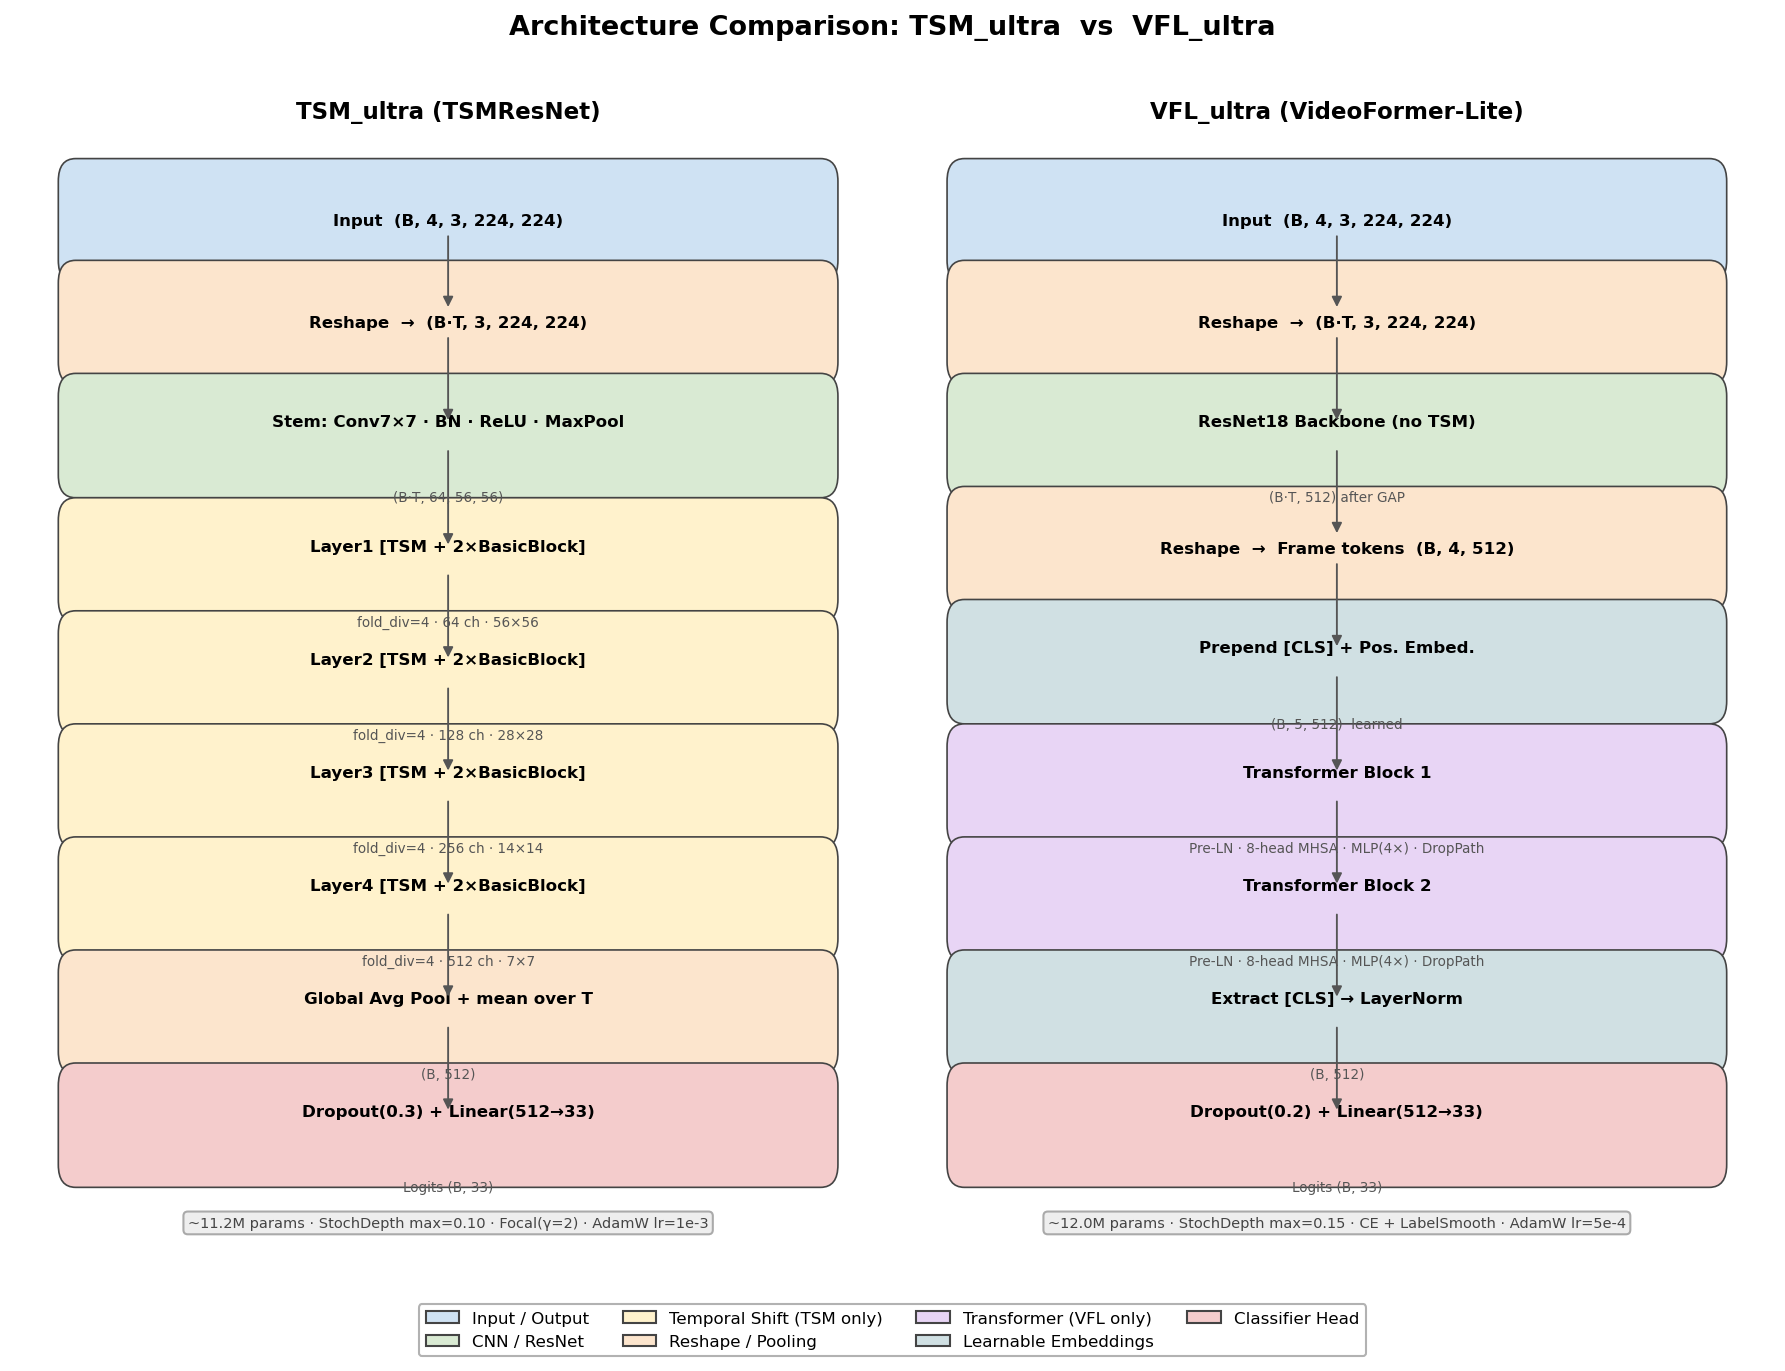
\includegraphics[width=\linewidth]{arch_comparison.png}
  \caption{The two complementary Track~A temporal mechanisms. \textbf{TSM} mixes
  time \emph{locally} via parameter-free channel shifts in every ResNet block,
  \emph{before} spatial pooling; \textbf{VideoFormer-Lite} mixes time
  \emph{globally} via \texttt{[CLS]}-token attention over pooled frame
  descriptors. The controlled comparison in Sec.~\ref{sec:abl} shows the former
  wins by $+3.0$\,pp at matched backbone size (Sec.~\ref{sec:trackA}).}
  \label{fig:arch}
\end{figure}

\begin{figure}[h]
  \centering
  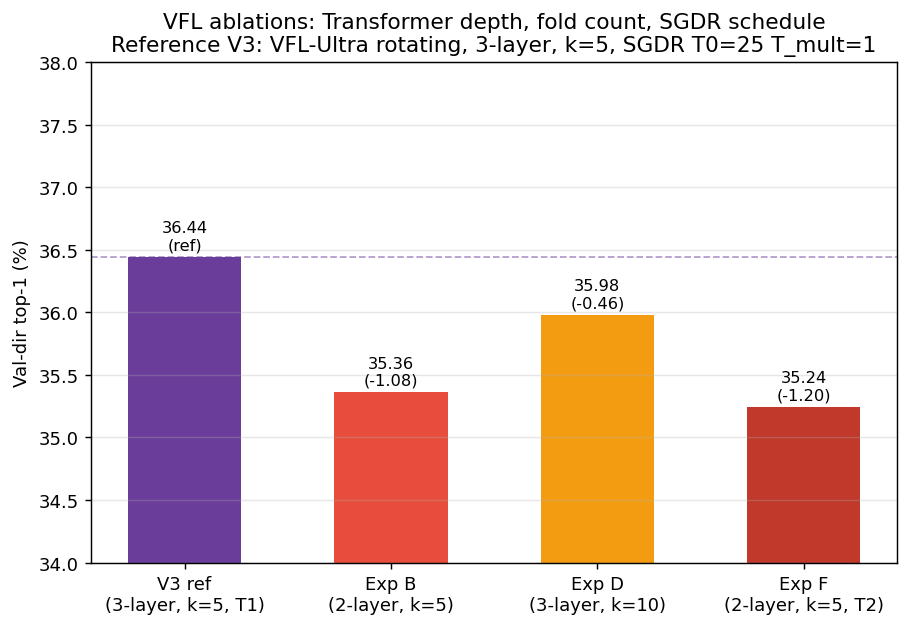
\includegraphics[width=\linewidth]{fig18_backbone_r18_vs_r50.png}
  \caption{TSM backbone and frame-count progression on \texttt{val\_dir}. The
  $T{=}8$ ResNet50 attempt regresses because interpolation duplicates frames;
  restoring $T{=}4$ and scaling to ResNet50 with rotating folds instead adds
  $+3.4$\,pp over the matched ResNet18, reaching the new single-model best of
  $42.85\%$ (Sec.~\ref{sec:trackA}).}
  \label{fig:backbone}
\end{figure}

\begin{figure}[h]
  \centering
  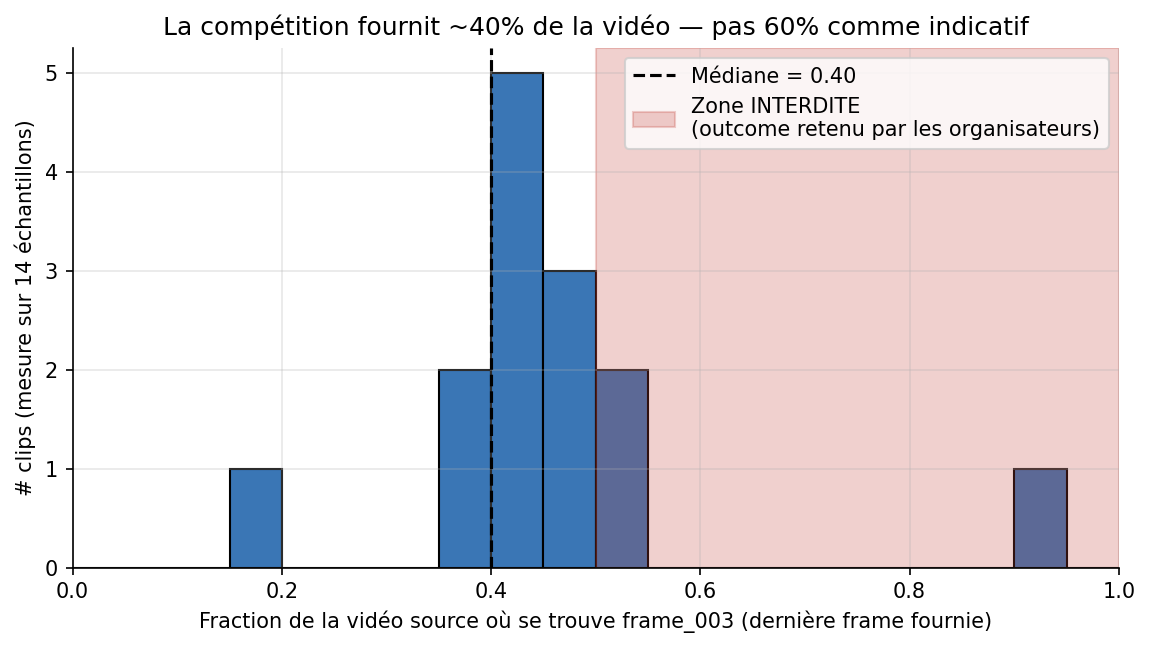
\includegraphics[width=\linewidth]{fig01_per_model_accuracy.png}
  \caption{Per-model \texttt{val\_dir} top-1/top-5 (Track~A). Correcting the
  frame count (TSM-Ultra$\rightarrow$TSM-Ultra-v2) and then scaling the
  backbone to ResNet50 (rotating folds) are the two largest per-model jumps;
  the $T{=}8$ ResNet50 scale-up regresses (Sec.~\ref{sec:results}).}
  \label{fig:permodel}
\end{figure}

\begin{figure}[h]
  \centering
  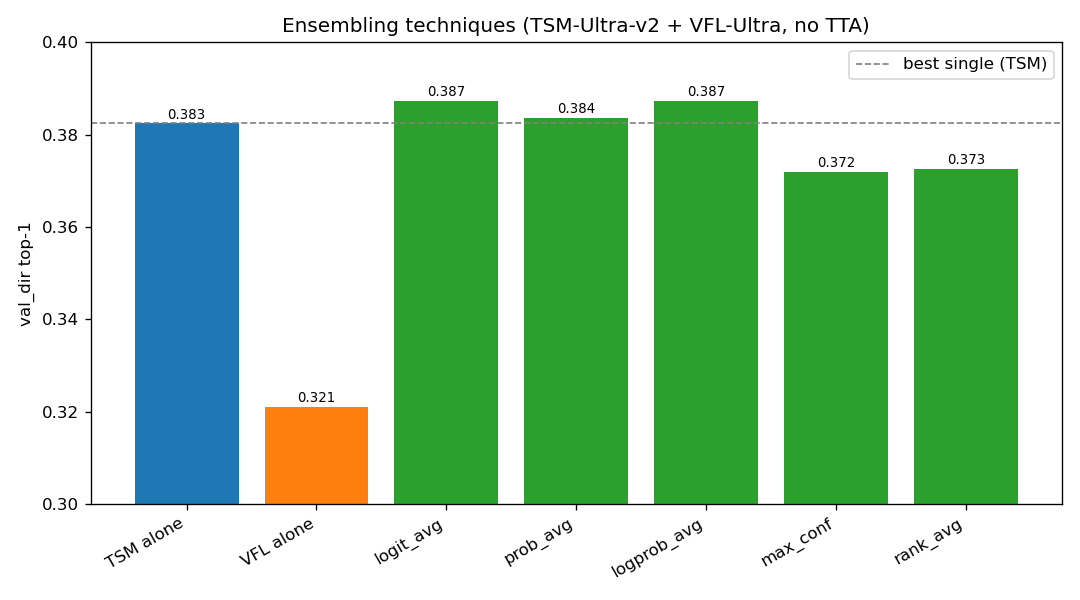
\includegraphics[width=\linewidth]{fig16_ablation_tsm.png}
  \caption{TSM ablations: focal-$\gamma$ sweep and SGDR restart shape (all
  other settings frozen). Any focal weight beats CE by ${\approx}0.5$\,pp;
  $\gamma{=}1$ and $\gamma{=}2$ are within noise; SGDR $T_\text{mult}$ has
  negligible effect ($<0.05$\,pp) (Sec.~\ref{sec:abl}).}
  \label{fig:abla_tsm}
\end{figure}

\begin{figure}[h]
  \centering
  
\includegraphics[width=\linewidth]{fig17_ablation_vfl.png}
  \caption{VFL ablations: Transformer depth (2 vs.\ 3 layers, $-1.08$\,pp for
  2 layers), fold count (5 vs.\ 10, $-0.46$\,pp for 10 folds --- VFL is
  data-saturated at $k{=}5$), and SGDR restart shape ($\leq 0.12$\,pp effect)
  (Sec.~\ref{sec:abl}).}
  \label{fig:abla_vfl}
\end{figure}

\begin{figure}[h]
  \centering
  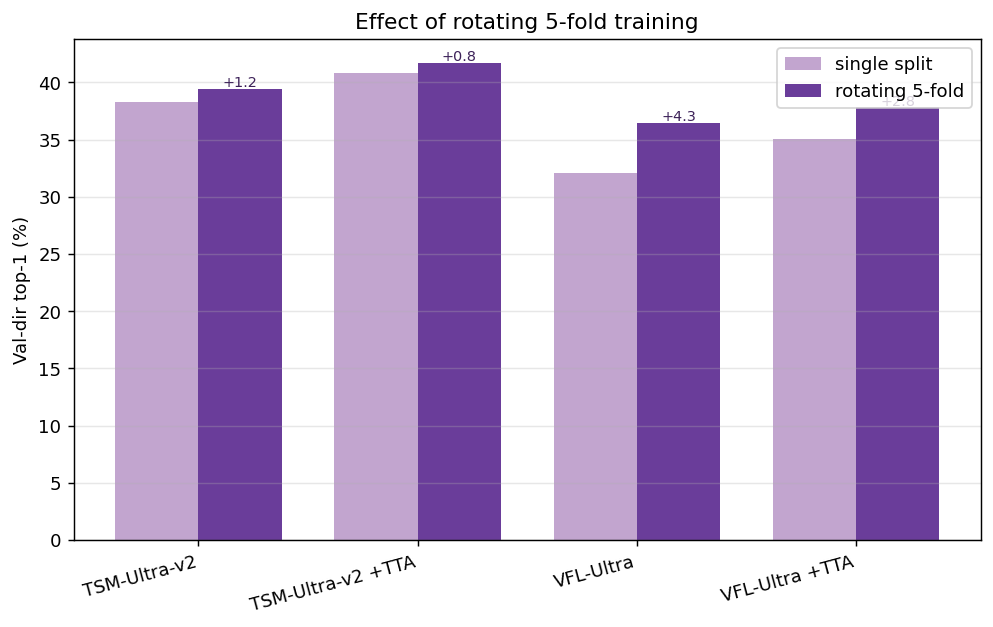
\includegraphics[width=\linewidth]{fig04_ensemble.png}
  \caption{Track~A ensemble vs.\ its components. Log-softmax late fusion of
  two TSM-ResNet18 variants, one VFL variant (all +TTA), the new
  TSM-ResNet50 and a CE-trained TSM ablation (no TTA) reaches $46.75\%$
  \texttt{val\_dir} and $0.4785$ public / $0.4547$ private on Kaggle ---
  our best closed-track submission (Sec.~\ref{sec:rotating}).}
  \label{fig:ensemble}
\end{figure}

\begin{figure}[h]
  \centering
  
\includegraphics[width=\linewidth]{fig11_leave_one_out.png}
  \caption{Track~A leave-one-out study on the 5-model ensemble
  (\texttt{val\_dir} top-1). The ResNet50 backbone is the dominant
  contributor ($-1.33$\,pp), ahead of the architecturally distinct VFL
  ($-0.64$\,pp): backbone diversity outweighs family diversity here
  (Table~\ref{tab:loo}).}
  \label{fig:loo}
\end{figure}

\begin{figure}[h]
  \centering
  
\includegraphics[width=\linewidth]{fig02_tta_effect.png}
  \caption{Effect of 10-crop spatial TTA on Track~A models. TTA adds
  ${\sim}1$\,pp on the strongest checkpoint and is essential at the ensemble
  level, where independent random errors from different crops average out
  (Sec.~\ref{sec:trackA}).}
  \label{fig:tta}
\end{figure}

\begin{figure}[h]
  \centering
  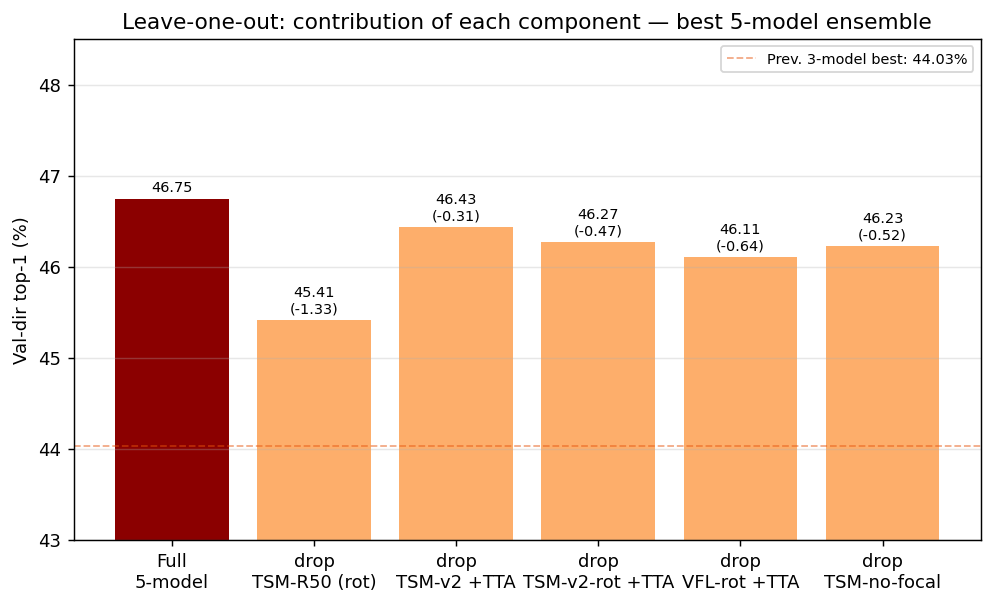
\includegraphics[width=\linewidth]{fig12_tta_directional_tradeoff.png}
  \caption{TTA directional-class trade-off. Horizontal-flip TTA improves most
  classes but hurts a few direction-encoded ones
  (\emph{Pulling left$\rightarrow$right} vs.\ \emph{right$\rightarrow$left})
  even after the flip-aware logit remap, because mirror evidence is
  intrinsically ambiguous when motion is short.}
  \label{fig:ttatradeoff}
\end{figure}

\begin{figure}[h]
  \centering
  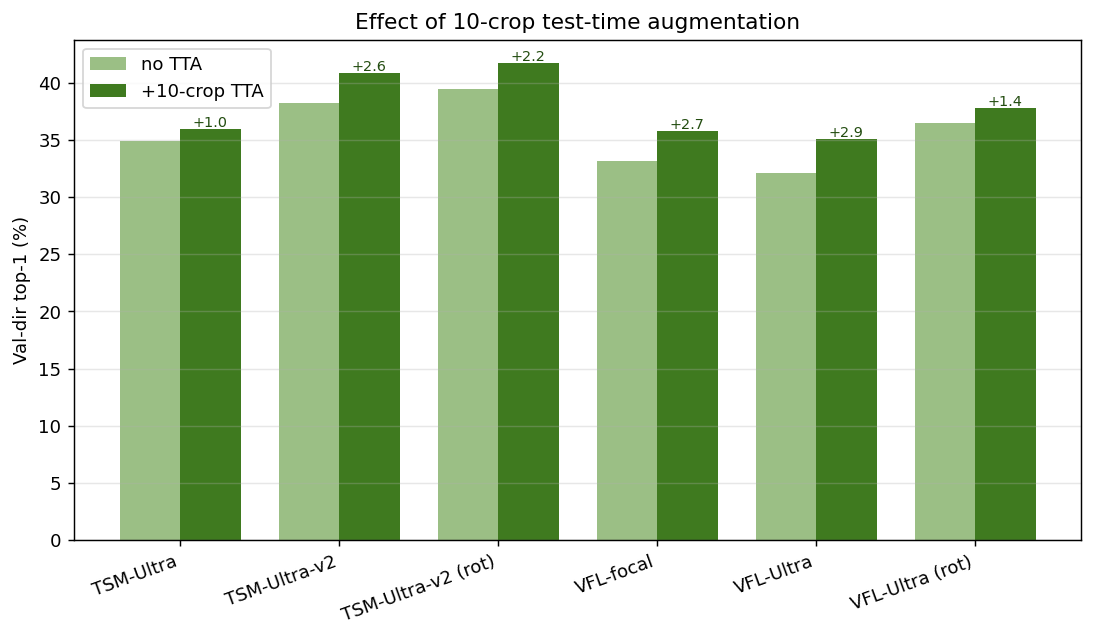
\includegraphics[width=\linewidth]{fig03_rotating_effect.png}
  \caption{Rotating-fold training. Re-training the strongest checkpoints on
  every train/val fold yields snapshots that share weights but disagree on the
  boundary, contributing uncorrelated errors that the log-softmax ensemble
  exploits; the gain is larger for VFL ($+4.3$\,pp) than for TSM ($+1.2$\,pp)
  (Sec.~\ref{sec:rotating}).}
  \label{fig:rotating}
\end{figure}

\begin{figure}[h]
  \centering
  
\includegraphics[width=\linewidth]{A_kaggle_journey.png}
  \caption{Track~B honest Kaggle progression. The discarded leaky submission
  ($0.81$, red) is plotted alongside every clean ensemble; each gain comes from
  adding architecturally distinct members, not from re-weighting. The dashed
  line marks the second-place public reference ($0.74$); the gap to it bounds
  what self-supervised pretraining + diverse ensembling buys us
  (Sec.~\ref{sec:results}, Table~\ref{tab:kaggle}).}
  \label{fig:kagglejourney}
\end{figure}

\begin{figure}[h]
  \centering
  
\includegraphics[width=\linewidth]{D_training_curves.png}
  \caption{V-JEPA progressive unfreezing + LLRD (Track~B internal val). Each
  phase warm-starts above the previous plateau: frozen probe ($0.55\!\to\!0.67$),
  then top-6 unfrozen + LLRD ($0.68\!\to\!0.71$), then full encoder
  ($0.70\!\to\!0.73$), then pseudo-label retrain ($0.72\!\to\!0.74$). The
  staircase pattern is the visual signature that LLRD has preserved each
  phase's feature geometry (Sec.~\ref{sec:trackB}).}
  \label{fig:vjepacurves}
\end{figure}

\begin{figure}[h]
  \centering
  
\includegraphics[width=\linewidth]{E_frame_position_histogram.png}
  \caption{Where shipped \texttt{frame\_003} sits in the source SSv2 clip
  (fraction). The dashed line at $0.40$ is the median end-of-window; the shaded
  region $[0.50,1.00]$ is the withheld outcome --- our re-extraction is
  hard-bounded to the un-shaded region (Sec.~\ref{sec:integrity}).}
  \label{fig:framehist}
\end{figure}

\begin{figure}[h]
  \centering
  
\includegraphics[width=\linewidth]{B_ensemble_size_vs_score.png}
  \caption{Track~B Kaggle vs.\ ensemble size. Returns from adding diverse
  honest members are still positive at $n{=}14$; at $n{=}6$, dropping K400
  + TSM \emph{hurts} despite their lower individual scores, because their
  uncorrelated errors disappear from the average
  (Table~\ref{tab:strategy}).}
  \label{fig:enssize}
\end{figure}

\begin{figure}[h]
  \centering
  
\includegraphics[width=\linewidth]{I_learned_weights_collapse.png}
  \caption{Learned ensemble weights collapse onto the two strongest members
  (${\sim}82\%$ of mass on \texttt{large\_attempt1\_top2} and
  \texttt{ssv2\_top1}), effectively zeroing K400 contributions. This is exactly
  why a learned weighting fails to beat uniform: it discards the very
  decorrelation signal that diverse weaker members provide
  (Sec.~\ref{sec:results}).}
  \label{fig:learnedw}
\end{figure}

\begin{figure*}[h]
  \centering
  
\includegraphics[width=0.95\textwidth]{fig05_per_class_f1.png}
  \caption{Per-class F1 (5-model ensemble, \texttt{val\_dir}). Directional
  single-object motions score highest; ``pretending'' and direction-ambiguous
  classes score lowest (Sec.~\ref{sec:failure}).}
  \label{fig:perclass}
\end{figure*}

\begin{figure*}[h]
  \centering
  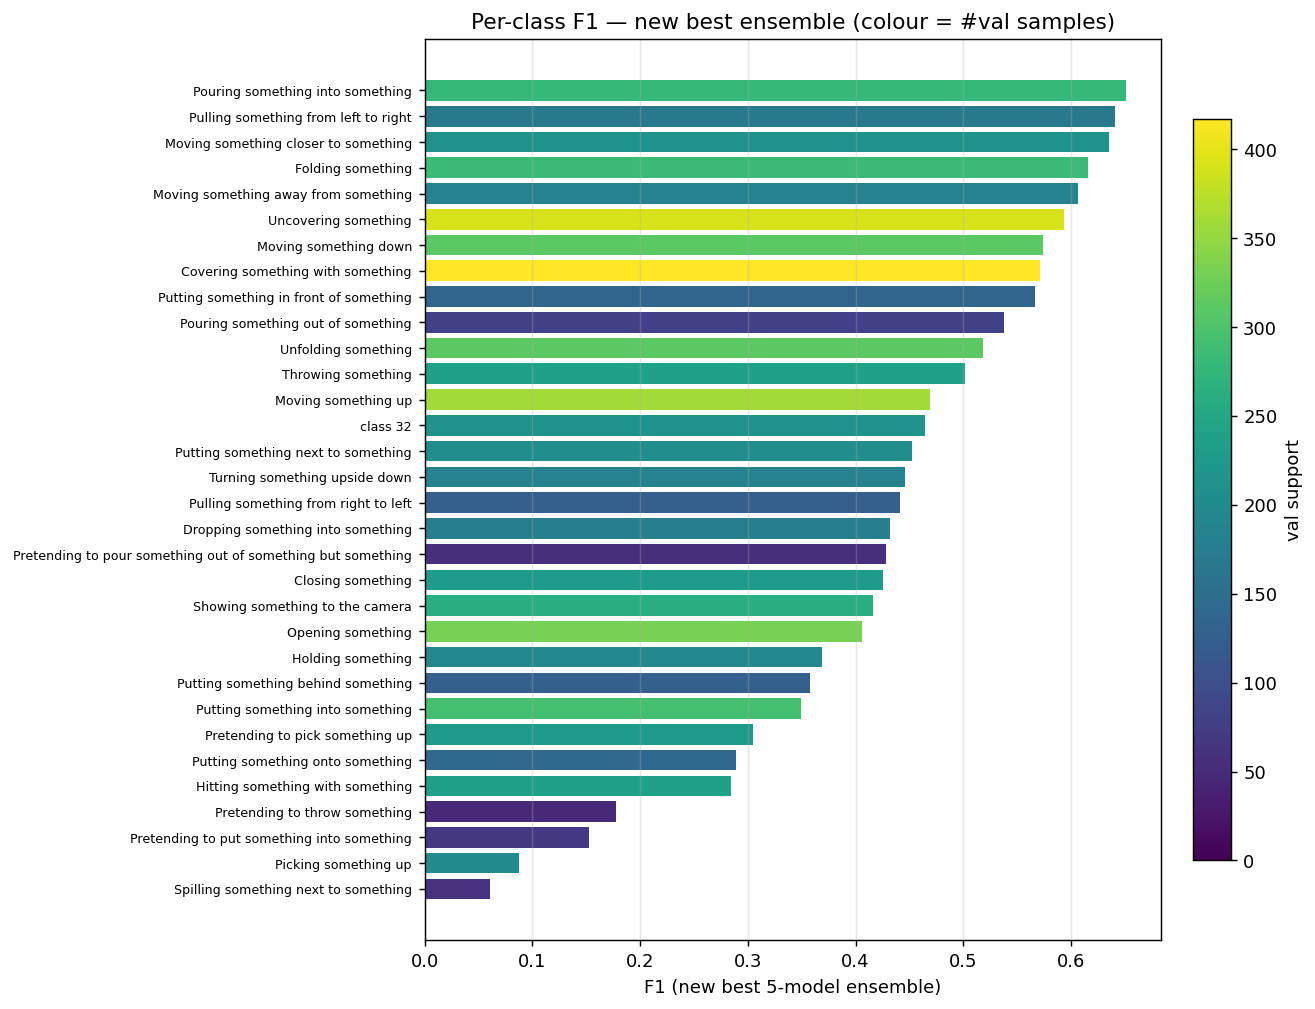
\includegraphics[width=0.95\textwidth]{fig06_confusion_matrix.png}
  \caption{$33\times33$ confusion matrix (5-model ensemble, \texttt{val\_dir}).
  Off-diagonal mass concentrates on semantically adjacent pairs (real vs.\
  pretended; fold vs.\ unfold; motion vs.\ \emph{holding}).}
  \label{fig:confmat}
\end{figure*}

\begin{figure*}[h]
  \centering
  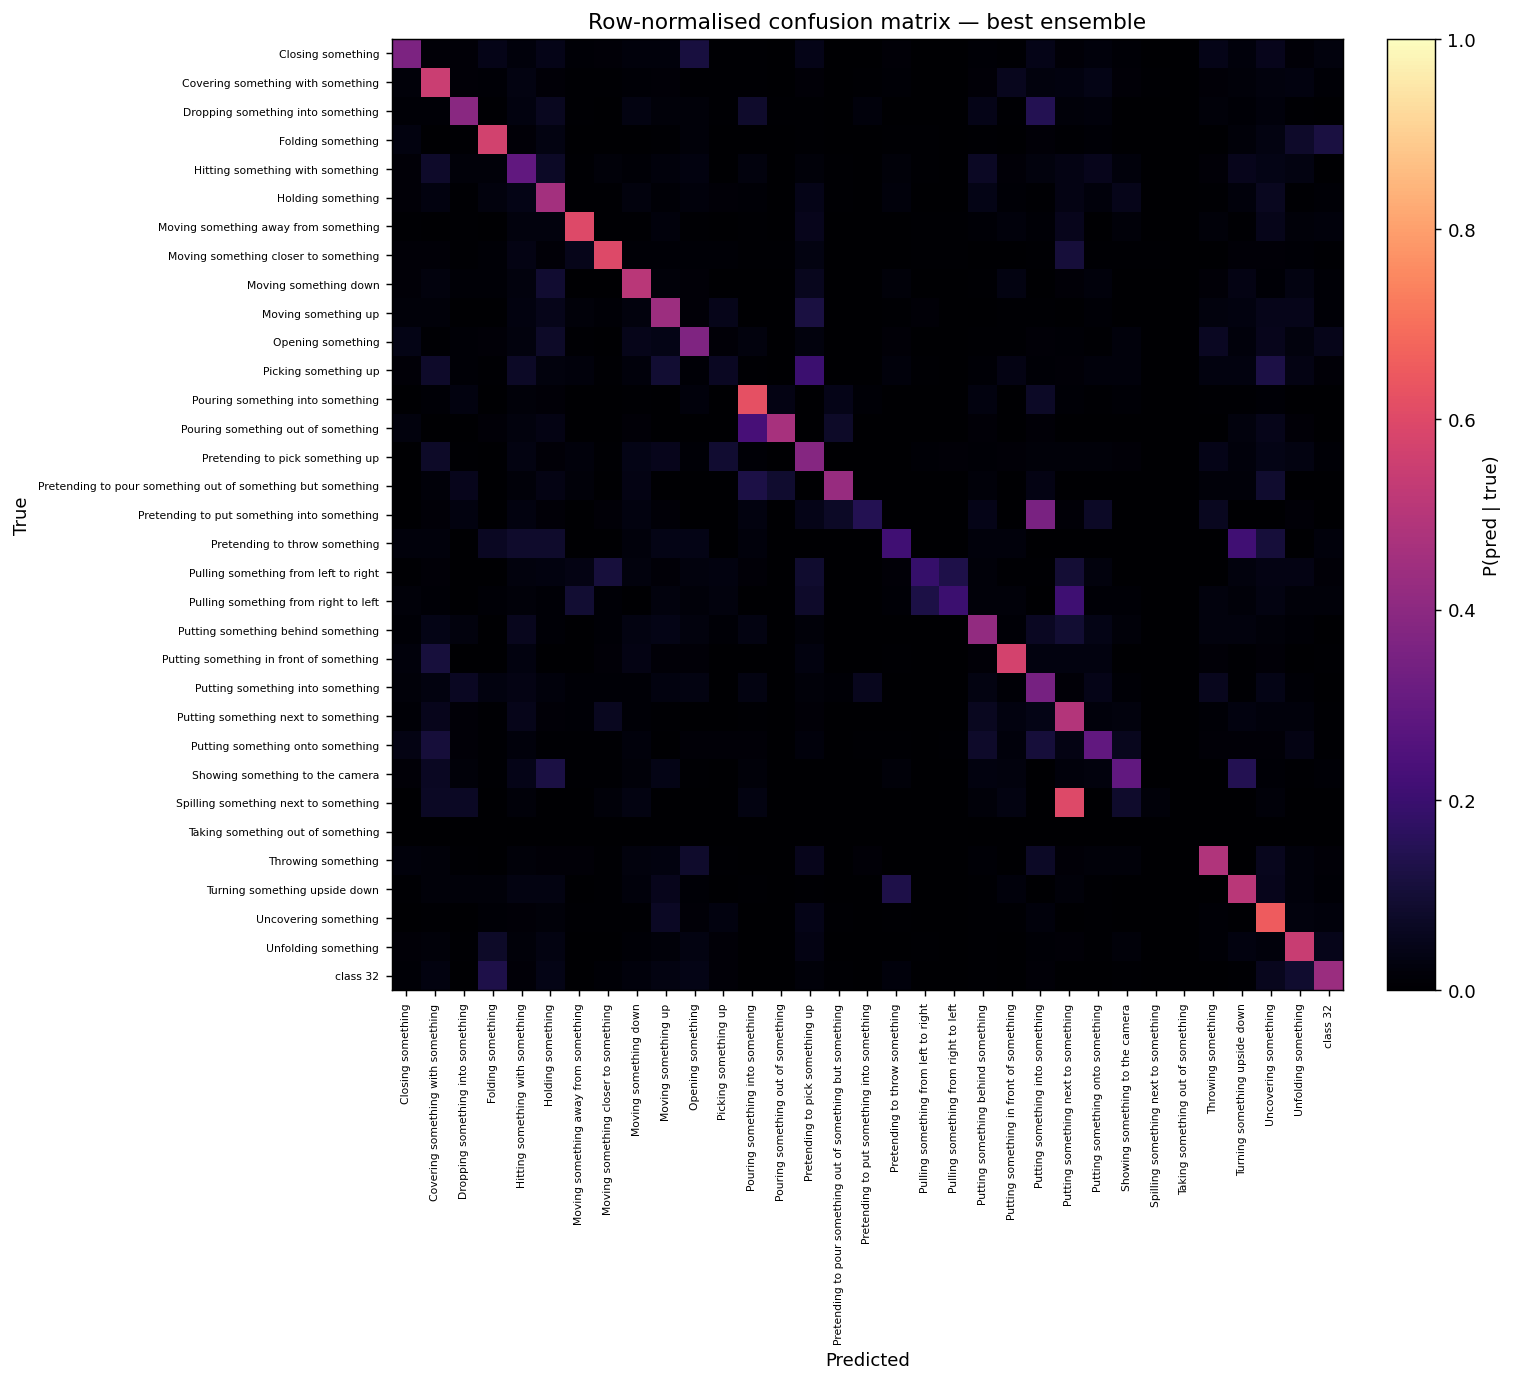
\includegraphics[width=0.95\textwidth]{fig07_confused_pairs.png}
  \caption{Most-confused class pairs. The dominant errors are intent (real vs.\
  pretended) and temporal-direction confusions (Sec.~\ref{sec:failure}).}
  \label{fig:pairs}
\end{figure*}

% =====================================================================
\clearpage
{\small
\bibliographystyle{ieeenat_fullname}
\bibliography{references}
}

\end{document}
